%!TEX root = ../main.tex

\chapter{Introduction}
\label{ch:introduction}

\dochaptoc % displays the toc of the chapter as margin note

\section{section name} % (fold)
\label{sec:section_name}

    \subsection{subsection name} % (fold)
    \label{sub:subsection_name}

        The tufte style book has no subsubsection, you may need to consider interplaying with \textsf{paragraphs\{paragraph name\}}

        \paragraph{paragraph name} % (fold)
        \label{par:paragraph_name}

            Or with the \textsf{newthought\{text\}} to write punchlines

            \newthought{New Thought,}
            you can learn more about the ways of using the Tufte's style at \href{https://tufte-latex.github.io/tufte-latex/}{https://tufte-latex.github.io/tufte-latex/}

        % paragraph paragraph_name (end)

    % subsection subsection_name (end)

% section section_name (end)

\section{Examples} % (fold)
\label{sec:examples}

    \newthought{Footnote/Sidenote} are equivalent
        \begin{itemize}
            \item \textsf{footnote[number][offset]\{text\}}:
                Footnote\footnote[314][1em]{regular footnote}
            \item \textsf{sidenote[number][offset]\{text\}}:
                Sidenote\sidenote[493][1em]{sidenote works as footnote}
        \end{itemize}

    \vspace{2em}

    \newthought{Marginnote}

        Use marginnote to write in the margin (offset is not possible)
        \marginnote{This is a margin note. Notice that there isn't a number preceding the note, and there is no number in the main text where this note was written.}

    \vspace{2em}
    \begin{equation}
        zaerze
        \mathnote{zerze}
    \end{equation}

    \vspace{2em}

    \newthought{Citations}

    \begin{itemize}
        \item \textsf{cite\{\}}: \cite{Tufte2006}
        \item \textsf{textcite[pre,][post]\{\}}: \textcite[pre,][post]{Tufte2006,Tufte1990,Bringhurst2005}
        \item \textsf{parencite[pre,][post]\{\}}: \parencite[pre,][post]{Tufte2006,Tufte1990,Bringhurst2005}
    \end{itemize}

    \lipsum[1]

    \begin{marginfigure}%[offset]
    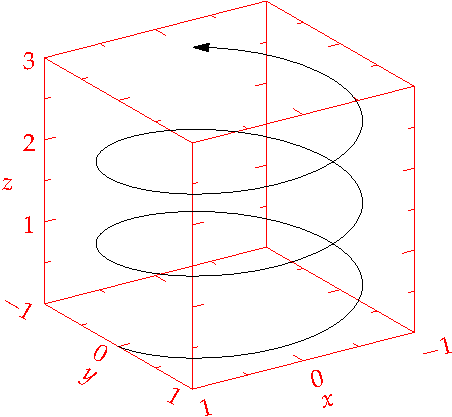
\includegraphics[width=\linewidth]{images/helix.pdf}
    \caption{margin figure}
    \label{app:fig:margin_fig}
    \end{marginfigure}

    \lipsum[1]

    \subsection{Figures} % (fold)
    \label{sub:figures}

    % subsection figures (end)

    \begin{figure}
        \centering
        \begin{subfigure}[b]{0.3\textwidth}
            \centering
            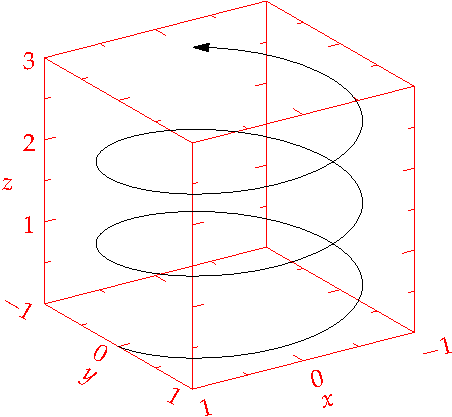
\includegraphics[width=\textwidth]{images/helix.pdf}
            \caption{subcaption 1}
            \label{fig:1}
        \end{subfigure}
        \hfill
        \begin{subfigure}[b]{0.3\textwidth}
            \centering
            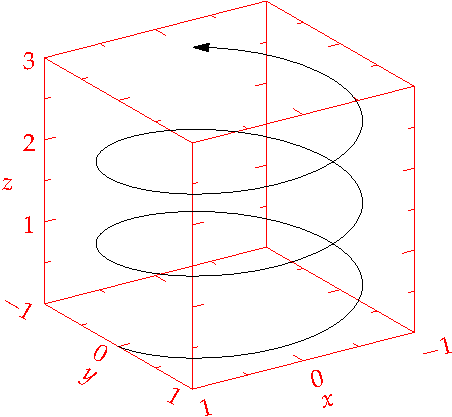
\includegraphics[width=\textwidth]{images/helix.pdf}
            \caption{subcaption 2}
            \label{fig:2}
        \end{subfigure}
        \hfill
        \begin{subfigure}[b]{0.3\textwidth}
            \centering
            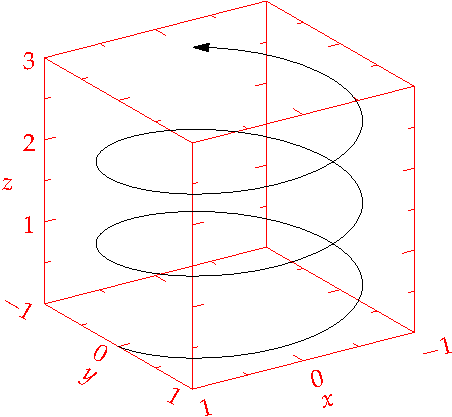
\includegraphics[width=\textwidth]{images/helix.pdf}
            \caption{subcaption 3}
            \label{fig:3}
        \end{subfigure}
        \caption{Example of figure with 3 subfigures}
        \label{fig:three_figs}
        % \setfloatalignment{b}  %b/t
        % \forceversofloat  % \forcerectofloat
    \end{figure}

    \begin{figure*}[h]
        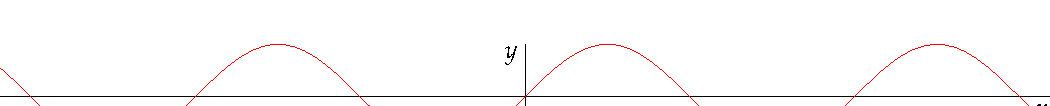
\includegraphics[width=\linewidth]{images/sine.pdf}%
        \caption{full width figure}%
        \label{app:fig:full_fig}%
    \end{figure*}

    \subsection{Equations} % (fold)
    \label{sub:equations}

        Normal equation
        \begin{equation}
        \label{eq:normal}
            \sum_{n=1}^{N} 1 / n \approx \ln(N).
        \end{equation}
        Full width equation
        \begin{fullwidth}
            \begin{equation}
            \label{eq:full_width}
                \sum_{n=1}^{N} 1 / n \approx \ln(N).
            \end{equation}
        \end{fullwidth}

        \newthought{There is also a custom command} \textsf{mathnote} to annotate equations.
        Its behavior is similar to \textsf{marginnote} but works in maths environments, like \textsf{equation} and \textsf{align}.
        I find it useful to make the transition between two steps of some derivations.
        Note that the equation number vanishes and the text is written in the margin.
        \begin{align}
            (x+1)^2
                &= (x+1)(x+1)
                \\
                &= x^2 + x + x + 1
                \quad\textsf{mathnote\{text\}\textbackslash\textbackslash}
                \mathnote{By developing the product}
                \\
                &= x^2 + 2x +1.
        \end{align}

        If you wish to preserve the equation number, you can combine the regular math environment with a manual teak of \textsf{marginnote} on a case-by-case basis.
        \marginnote{\text{ }\\[0.3em]Annotation}
        \begin{equation}
            \label{eq:annotated}
            \pi \approx 3.14
        \end{equation}

    % subsection equations (end)

    \subsection{Nomenclature, Glossary, Accronyms} % (fold)
    \label{sub:nomenclature_glossary_accronyms}

        \newthought{Indices}
            Fruits\index{fruits}, e.g.,
            orange\index{fruits!orange},
            banana\index{fruits!banana}
            apple\index{fruits!apple},
            kiwi\index{fruits!kiwi}

        \newthought{Acronyms}
            acrshort: \acrshort{gcd}, \acrshort{dpp}
            acrlong: \acrlong{gcd}, \acrlong{dpp}

        \newthought{Glossary}
            \Gls{tomato} \gls{tomato}
            \Glspl{tomato} \glspl{tomato}\\
            \Gls{dpp} \gls{dpp}

    % subsection nomenclature_glossary_accronyms (end)

% section examples (end)

\clearpage

\newthought{Below is a list of our contributions.}

\begin{fullwidth}
\textit{Journal paper(s)} % (fold)
% \label{par:journals}
    \begin{quote}
      \begin{itemize}
        \item[\paperIcon] \fullcite{Tufte2006}.
      \end{itemize}
    \end{quote}
\end{fullwidth}
% paragraph journals (end)

\begin{fullwidth}
\textit{Submitted to a journal} % (fold)
\label{par:working paper}
    \begin{quote}
      \begin{itemize}
        \item[\paperIcon] \fullcite{Tufte2006}.
      \end{itemize}
    \end{quote}
\end{fullwidth}
% textit working paper (end)

\begin{fullwidth}
\textit{Conference papers} % (fold)
\label{par:conferences}
    \begin{quote}
      \begin{itemize}
        \setlength{\itemsep}{5pt}
        \item[\conferenceIcon] \fullcite{Tufte2006}.
        \item[\conferenceIcon] \fullcite{Tufte2006}.
      \end{itemize}
    \end{quote}
\end{fullwidth}
% textit conferences (end)

\begin{fullwidth}
\textit{Workshop papers} % (fold)
\label{par:workshops}
    \begin{quote}
      \begin{itemize}
        \setlength{\itemsep}{5pt}
        \item[\conferenceIcon] \fullcite{Tufte2006}.
        \item[\conferenceIcon] \fullcite{Tufte2006}.
      \end{itemize}
    \end{quote}
\end{fullwidth}
% textit workshops (end)

\section{Outline of the manuscript} % (fold)
\label{sec:outline}

    \newthought{The manuscript is divided into five chapters.}

    \newthought{Chapter~\ref{ch:chapter_1}}
        lays the ground material for the subsequent chapters.

    \newthought{Chapter~\ref{ch:chapter_2}}
        discusses several methods available to

    \newthought{Chapter~\ref{ch:chapter_3}}
        discusses various methods to

    \newthought{Chapter~\ref{ch:chapter_4}}
        includes material accepted to

    \newthought{Chapter~\ref{ch:chapter_5}}
        includes material submitted to

    \newthought{The final section}
        contains a discussion

% section outline (end)

% chapter introduction (end)
